\documentclass{article}
\usepackage[legalpaper, left=1 cm, right=1cm, top=0.5cm, bottom=0.5cm] {geometry}
\date{} % Remove a exibição da data
\usepackage{xcolor}
\usepackage{listings}
\usepackage{graphicx}
\usepackage{hyperref} % Para criar links
\usepackage[utf8]{inputenc}
\usepackage[T1]{fontenc}

    \lstset{
    language=python,
    basicstyle=\ttfamily,
    keywordstyle=\bfseries\color{blue},
    commentstyle=\color{blue},
    stringstyle=\color{red!70!black},
    numberstyle=\tiny,
    stepnumber=1,
    numbersep=5pt,
    backgroundcolor=\color{white},
    breaklines=true,
    breakautoindent=true,
    showspaces=false,
    showstringspaces=false,
    showtabs=false,
    tabsize=2,
    literate={~}{{\textasciitilde}}1, % Trata ~ como um caractere normal
    extendedchars=true, % Permite caracteres estendidos (acentos, etc.)
    inputencoding=utf8, % Define a codificação de entrada como UTF-8
    literate={á}{{\'a}}1 {ã}{{\~a}}1 {ç}{{\c{c}}}1
    }

\title{Listas cengel} 
\begin{document}
\maketitle
\tableofcontents
\setlength{\parindent}{8pt}
\noindent\rule{\textwidth}{0.4pt}


\newpage
\section{Introdução}
\textbf {Questões conceituais (C):
$2, 4-6, 14-21, \quad 23 \quad , 25-27 \quad , \quad 30$}\\
\textbf{Problemas:
7, 8, 28, 43, 70, 78, 84
}
\begin{itemize}
    \item \textcolor{red}{
     1.4 - Um recipiente contendo água líquida é colocado em um congelador e é resfriado de 20 °C para –5 °C. Identifique o(s) fluxo(s) de energia e a acumulação de energia de tectados no processo e explique as mudan- ças que ocorrem}\\
    resp energia é retirada da agua , até que tal atinja a temperatura de 0° , na qual ocorre a transição de estado.
    \textbf{Resposta chatgpt}
    No processo descrito, onde um recipiente contendo água líquida é resfriado de 20 °C para -5 °C em um congelador, ocorrem vários fluxos de energia e acumulações de energia. Aqui está uma correção e uma explicação mais detalhada:

Fluxo de Energia: Durante o resfriamento da água, há transferência de energia térmica do sistema (água) para o ambiente (ar dentro do congelador). Esse processo ocorre porque a temperatura do ambiente é mais baixa do que a temperatura da água, resultando em uma transferência líquida de calor do sistema para o ambiente. Esse é o principal fluxo de energia no processo.

Acumulação de Energia: Conforme a água perde energia térmica, sua temperatura diminui. No entanto, quando a água atinge 0 °C, ocorre uma mudança de fase, onde a água líquida se transforma em gelo sólido. Durante essa transição de fase, mesmo que a temperatura permaneça constante a 0 °C, há uma acumulação de energia na forma de energia latente de fusão, que é a energia necessária para mudar a fase da água de líquida para sólida sem alterar sua temperatura.

Então, a correção seria: Energia é retirada da água enquanto ela está sendo resfriada, até que atinja a temperatura de 0 °C, na qual ocorre a transição de estado e há acumulação de energia na forma de energia latente de fusão.

    \noindent\rule{\textwidth}{0.4pt}
    \item \textcolor{red}{1 .5A massa específica das fibras, dos isolamentos térmicos, das espumas isolantes e do algodão é pequena. Por que isso ocorre?}\\
    a baixa massa específica desses materiais está relacionada à sua porosidade, composição leve, finalidade específica de isolamento e características desejáveis para certas aplicações. Essa leveza é uma propriedade valiosa em contextos nos quais é importante minimizar o peso ou melhorar as propriedades isolantes.\\
    \noindent\rule{\textwidth}{0.4pt}
    \item \textcolor{red}{1 .6 A massa específica é a única medida de como a massa é distribuída em um volume? O valor da massa específica pode variar de um ponto para outro?}\\
    resp :Não, a massa específica não é a única medida. A massa específica é uma medida que relaciona a massa de um material ao seu volume. No entanto, a distribuição de massa em um objeto também pode ser afetada por sua densidade ou mesmo por sua geometria. Outras propriedades, como densidade linear ou superficial, podem ser relevantes dependendo da situação.Geralmente, a massa específica é considerada uma propriedade intensiva, o que significa que ela é uniforme em todo o material, independentemente do tamanho ou da quantidade do material examinado. Entretanto, se houver variação na composição ou na densidade do material, a massa específica pode variar em diferentes partes do objeto. Portanto, a resposta "Sim" é válida se houver heterogeneidade na distribuição de massa.
    
\end{itemize}
\noindent\rule{\textwidth}{0.4pt}
\subsection{cengel}
\subsubsection{cengel 7.ed}
\subsection*{1-2Uma das coisas mais divertidas que uma pessoa pode fazer é verificar que, em certas partes do mundo, um carro em ponto morto desloca-se para cima quando os freios são liberados. Tais ocorrências são até mesmo transmitidas pela TV. Isso pode realmente acontecer ou é uma ilusão de ótica? Como você pode verificar se uma estrada está realmente em aclive ou declive?}
A sensação de um carro em ponto morto deslocando-se para cima quando os freios são liberados em uma estrada aparentemente plana é uma ilusão de ótica conhecida como ilusão de subida. Isso geralmente ocorre em estradas que têm uma inclinação descendente, mas devido ao relevo ao redor ou à orientação da estrada, pode parecer que o carro está subindo.

Para verificar se uma estrada está realmente em aclive ou declive, você pode usar alguns métodos simples:

\textbf{Nível de bolha}: Utilize um nível de bolha, que é um instrumento que indica se uma superfície está nivelada. Coloque o nível em uma superfície plana na estrada, como o capô do carro, e observe a posição da bolha. Se a bolha estiver centrada, a superfície está nivelada. Se estiver inclinada para frente, a estrada está em declive; se estiver inclinada para trás, a estrada está em aclive.

\textbf{Observação visual}: Olhe para o horizonte e pontos de referência ao redor. Se houver uma inclinação visível na paisagem ou nos objetos ao lado da estrada, isso pode indicar a inclinação real da estrada.

\textbf{Utilização de aplicativos e dispositivos:} Existem aplicativos para smartphones e dispositivos como inclinômetros que podem medir a inclinação de uma superfície. Coloque o dispositivo em uma parte plana da estrada e observe a leitura.

É importante notar que, em algumas situações, a inclinação pode ser sutil e difícil de detectar visualmente. Além disso, a ilusão de subida pode persistir em algumas condições específicas. No entanto, esses métodos devem ajudar a determinar com precisão se a estrada está em aclive, declive ou é plana.\\

\noindent\rule{\textwidth}{0.4pt}
\subsection*{1-4 Em um artigo, afirma-se que um motor turbofan recentemen- te desenvolvido produz 15.000 libras de empuxo para impulsionauma aeronave para a frente. A medida considerada aqui é lbm ou lbf? Explique.} é usada libra força já que é a unidade inglesa para força

\textbf{correção chat gpt chatgpt}\\ Sim, sua interpretação está correta. A afirmação menciona que o motor turbofan produz 15.000 libras de empuxo. Nesse contexto, "libras" está se referindo a libras-força (lbf), que é a unidade de força no sistema de medidas inglês.

É importante destacar a diferença entre libras-força (lbf) e libras-massa (lbm):

Libra-força (lbf): É a unidade de medida de força no sistema inglês. Representa a força exercida pela gravidade em uma massa de uma libra. Quando você diz que o motor turbofan produz 15.000 libras de empuxo, está se referindo a 15.000 libras-força.

Libra-massa (lbm): É a unidade de medida de massa no sistema inglês. Representa a quantidade de matéria em uma libra. Se a medida fosse em libras-massa, a expressão seria diferente.

Portanto, a medida de empuxo de 15.000 libras no contexto do artigo está em libras-força.\\
\noindent\rule{\textwidth}{0.4pt}
\subsection*{1–5C Explique por que o ano-luz tem a dimensão de comprimento} a unidade Ano-luz se refere a o espaço em que a luz se desloca em um ano

\noindent\rule{\textwidth}{0.4pt}
\subsection*{1-14Em algum estágio da solução de um problema, uma pessoa acabou chegando à equação E  25 kJ + 7 kJ/kg. Aqui, E é a ener- gia total e tem como unidade o quilojoule. Determine como corrigir o erro e discuta o que o causou.}
Parece que A pessoa tentava somar duas unidades diferentes , para fornecer uma possivel soliução seria necessario a massa total , e assim fazer um interpolação para enegia a que se faz referencia.\\
\noindent\rule{\textwidth}{0.4pt}


\subsection*{1–23C O peso de um sistema é uma propriedade intensiva ou extensiva?}pela expressão $m \cdot\vec{g} $ que caracteriza a expressão matematica para o peso, o peso depende da massa, portanto é uma propriedade extensiva
\textbf{resposta chatgt\\O peso de um sistema é uma propriedade extensiva. Propriedades extensivas são aquelas que dependem da quantidade de matéria presente no sistema. O peso de um sistema é uma medida da força gravitacional exercida sobre ele e está diretamente relacionado à quantidade de matéria presente, ou seja, à massa do sistema.
Por exemplo, se você tiver dois objetos idênticos, o peso total do sistema será o dobro do peso de apenas um dos objetos. Isso ocorre porque o peso é uma propriedade que se soma quando mais matéria é adicionada ao sistema, o que é uma característica das propriedades extensivas.}\\
\noindent\rule{\textwidth}{0.4pt}
\subsection*{1–25C Para que um sistema esteja em equilíbrio termodinâmico, a temperatura e a pressão precisam ser as mesmas em todos os lugares?}
Para que um sistema esteja em equilibrio é necessario que a temperatura seja a mesma em todas as partes do sistema.Porém a presão pode variar com a altura, mas ainda assim deve estar em equilíbrio em todas as regiões do sistema.\\
\noindent\rule{\textwidth}{0.4pt}
\subsection*{1–26C O que é um processo de quase-equilíbrio? Qual é a sua importância na engenharia?}
Um processo de quase equilibrio pode ser visto como um processo lento o suficiente para o sistema mude de  forma  uniforme em toda sua extensão , ajustando internamente para que suas propriedades de uma parte do sistema nao mudem mais rapidamente do que as propriedades da soutras parte \\
\noindent\rule{\textwidth}{0.4pt}
\subsection*{1-27CDefina os processos isotérmico, isobárico e isocórico.}
\begin{itemize}
    \item Isotérmico - Processo no qual o sistema não altera sua temperatura  ao no decorrer
    \item Isobárico - processoa no qual a pressão se mantem constante
    \item Isocórico - processo no qual o volume se mantém constante e as outras duas propriedades variam.
\end{itemize}
\noindent\rule{\textwidth}{0.4pt}
\subsection*{1-28  O que é o postulado de estado?}
segundo o postulado de estado um sistema compressivel simples é completamente especificado por duas propriedades intensivas independentes.
\subsection*{1-30Ao analisar a aceleração de gases à medida que eles escoam por um bocal, o que você escolheria como seu sistema? Que tipo de sistema é esse?}
o sistema seria o fluido que escoa pelo bocal em determinado periodo em regime permanente
\textbf{Eu escolheria o conjunto formado pelo bocal e pelos gases escoando através dele como meu sistema de interesse. Esse tipo de sistema é conhecido como um sistema de controle de volume ou um sistema aberto. Isso ocorre porque há uma entrada e uma saída de massa (os gases) através do bocal, e as propriedades do sistema podem mudar ao longo do tempo devido a esse fluxo de massa. Ao analisar a aceleração dos gases à medida que eles passam pelo bocal, é importante considerar as interações entre o bocal e os gases, bem como as mudanças nas propriedades dos gases ao longo do processo de escoamento.
}\\
\noindent\rule{\textwidth}{0.4pt}
\subsection*{1-31O que é um processo com escoamento em regime permanente?}
processo durante o qual um fluido escoa através de um volume de controle de forma permanente 
Correção: Um processo durante o qual um fluido escoa através de um volume de controle de forma permanente.

Um processo com escoamento em regime permanente ocorre quando as propriedades do fluido e as condições de escoamento em um sistema não variam com o tempo. Isso significa que as propriedades do fluido, como velocidade, pressão e temperatura, permanecem constantes em qualquer ponto ao longo do tempo. Em outras palavras, o fluxo de fluido através de um volume de controle é constante e não muda com o tempo. Este tipo de processo é comumente encontrado em sistemas de engenharia, como em tubulações de água, dutos de ar condicionado e em muitos processos industriais onde o fluxo é estável e não há variações significativas ao longo do tempo.\\
\noindent\rule{\textwidth}{0.4pt}
\subsection*{1–33C O que é a lei zero da termodinâmica?}
A Lei em questão afirma que se dois corpos estão em equilibrio termico entre si , eles estão em equilibrio termico com um terceiro

\subsubsection{cengel 5.ed}
\subsection*{$1-2$Por que um ciclista ganha velocidade em uma descida mesmo quando não está pedalando? Isso viola o princípio da conservação da energia?}
Quando um ciclista está descendo uma colina e ganhando velocidade sem pedalar, a energia potencial gravitacional que o ciclista tinha no topo da colina está sendo convertida em energia cinética à medida que ele desce.

No topo da colina, o ciclista tem uma alta energia potencial devido à sua altura em relação ao solo. Conforme ele desce, essa energia potencial é transformada em energia cinética, que está associada ao movimento do ciclista. De acordo com o princípio da conservação de energia, a soma total de energia (energia potencial mais energia cinética) permanece constante, desde que não haja dissipação de energia por forças como o atrito do ar ou a resistência dos pneus.
Assim, a ganho de velocidade do ciclista em uma descida sem pedalar não viola o princípio da conservação de energia, pois a energia está apenas mudando de uma forma para outra. A energia total do sistema (ciclista mais bicicleta) permanece a mesma, apenas a distribuição entre energia potencial e cinética está mudando à medida que o ciclista se move.\\

\noindent\rule{\textwidth}{0.4pt}
\subsection*{1-3Um funcionário de escritório afirma que uma xícara de café frio em sua mesa aqueceu até $80^\circ C$ ao captar energia do ar circundante, que está a $25^\circ C$. Existe alguma verdade em sua afirmação? Este processo viola alguma lei termodinâmica}
Não existe verdade nessa afirmação , pois depndendo de sua temperatura inicial , o café elevaria sua temperatura até se igualar a temperatura ambiente, ou seja até os $25^\circ C$  \\
\textbf{complemento chatgpt}
Isso violaria as leis da termodinâmica, especificamente a lei zero da termodinâmica, que estabelece que dois corpos em equilíbrio térmico com um terceiro corpo estão em equilíbrio  entre si. Portanto, a temperatura final do café após alcançar o equilíbrio  com o ar circundante seria $25^\circ C$.
\noindent\rule{\textwidth}{0.4pt}\\
\subsection*{$1-15$Uma grande fração da energia térmica gerada no motor de um carro é rejeitada para o ar pelo radiador através da +água circulante. O radiador deve ser analisado como sistema fechado ou como sistema aberto? Explicar.}

um sistema aberto pois envolve um fluxo de massa saindo 
\textbf{complemento chat gpt}
Um sistema aberto pois envolve um fluxo de massa saindo.

A energia térmica gerada no motor do carro é transferida para a água circulante, que por sua vez, é levada para o radiador, onde essa energia térmica é dissipada para o ar circundante. O processo de dissipação envolve a transferência de calor do líquido (água) para o meio ambiente (ar), e como há um fluxo contínuo de água entrando e saindo do radiador para transferir calor, o sistema não pode ser considerado isolado. Portanto, o radiador deve ser analisado como um sistema aberto, já que há um fluxo de massa (água) saindo dele.
\subsection*{1-16Uma lata de refrigerante em temperatura ambiente é colocada na geladeira para esfriar. Você modelaria a lata de refrigerante como um sistema fechado ou como um sistema aberto? Explicar.} É um sistema fechado pois há apenas trocar de calor com a vizinhança, e não troca de massa 
É um sistema fechado pois há apenas troca de calor com a vizinhança, e não troca de massa.

Quando uma lata de refrigerante é colocada na geladeira para esfriar, não há entrada ou saída de matéria da lata. O único processo que ocorre é a transferência de calor entre o refrigerante dentro da lata e o ambiente da geladeira. Não há fluxo de matéria entrando ou saindo da lata durante esse processo, apenas uma transferência de energia na forma de calor. Portanto, a lata de refrigerante pode ser modelada como um sistema fechado, pois não há troca de massa com a vizinhança, apenas troca de calor.
\subsection*{1–17C Qual é a diferença entre propriedades intensivas e extensivas?}
propriedades intensivas não dependem da extensão do sistema , porém as extensivas sim , como ser um propriedade extensiva e pressão uma propriedade intensiva
\begin{itemize}
    \item Propriedades Intensivas: São aquelas que não dependem da quantidade de matéria presente no sistema. Em outras palavras, elas permanecem as mesmas, independentemente do tamanho ou da quantidade de substância no sistema. Exemplos comuns incluem temperatura, pressão, densidade, ponto de ebulição e ponto de fusão.

    \item Propriedades Extensivas: São aquelas que dependem da quantidade de matéria presente no sistema. Elas variam de acordo com o tamanho ou a quantidade de substância no sistema. Exemplos incluem massa, volume, energia total, entalpia total e número de mols.
    
    
\end{itemize}
Um exemplo clássico para diferenciar esses conceitos é comparar a massa e a densidade. A massa é uma propriedade extensiva, pois depende da quantidade de matéria presente (quanto mais matéria, maior a massa). Por outro lado, a densidade é uma propriedade intensiva, pois não importa quanto da substância está presente, a densidade permanece constante para aquela substância específica nas mesmas condições de temperatura e pressão.
\subsection*{1-23 O que é um processo de fluxo constante?}Em um regime simples , é um processo em que a quantidade de massa que entra é igual a massa que sai.\\
\textbf{chatgpt}\\
Um processo de fluxo constante é, de fato, um processo em que a quantidade de massa (ou volume, em certos casos) que entra em um sistema é igual à quantidade que sai durante um período de tempo específico. Essa constância de fluxo pode se referir a diferentes variáveis, como massa, volume, energia, entre outras.

Em sistemas de engenharia ou processos industriais, um exemplo comum de processo de fluxo constante é o fluxo de fluidos em tubulações, onde a vazão de entrada do fluido é igual à vazão de saída, mantendo assim um fluxo constante ao longo do tempo. Isso é essencial para garantir um funcionamento estável e eficiente do sistema.
\subsection*{1-27Quais são as escalas de temperatura ordinária e absoluta no SI e no sistema inglês?}
As escalas de temperatura ordinária e absoluta são medidas de temperatura comuns em diferentes sistemas de unidades, como o Sistema Internacional (SI) e o sistema inglês. Aqui estão as escalas de temperatura ordinária e absoluta em ambos os sistemas:

No Sistema Internacional (SI):\\

Escala de temperatura ordinária: Celsius (°C)\\
Escala de temperatura absoluta: Kelvin (K)\\
No sistema inglês:\\

Escala de temperatura ordinária: Fahrenheit (°F)\\
Escala de temperatura absoluta: Rankine (°R)\\
Na escala Celsius (°C), o ponto de congelamento da água é 0°C, enquanto o ponto de ebulição é 100°C sob pressão atmosférica normal ao nível do mar. Na escala Fahrenheit (°F), o ponto de congelamento da água é 32°F, enquanto o ponto de ebulição é 212°F sob as mesmas condições.\\

A escala Kelvin (K) é uma escala absoluta em que zero absoluto (0 K) representa a ausência total de energia térmica, e cada grau kelvin tem o mesmo tamanho que um grau Celsius. A escala Rankine (°R) é semelhante à escala Kelvin, mas é usada no sistema inglês. Zero Rankine (0 °R) é equivalente ao zero absoluto, e o tamanho dos graus Rankine é o mesmo que os graus Fahrenheit.\\

\subsection*{Considere um termômetro de álcool e de mercúrio que marca exatamente 0°C no ponto de gelo e 100°C no ponto de vapor. A distância entre os dois pontos é dividida em 100 partes iguais em ambos os termômetros. Você acha que esses termômetros darão exatamente a mesma leitura a uma temperatura de, digamos, 60°C? Explicar.}
Embora ambos os termômetros estejam divididos em 100 partes iguais entre os pontos de congelamento e vapor, o álcool e o mercúrio têm diferentes coeficientes de expansão térmica, o que afeta a maneira como eles respondem às mudanças de temperatura.

O mercúrio tem um coeficiente de expansão térmica menor do que o álcool, o que significa que o mercúrio se expande ou contrai menos para uma dada mudança de temperatura em comparação com o álcool. Isso resulta em uma resposta diferente dos dois termômetros para uma mesma temperatura.

Suponha que ambos os termômetros marquem exatamente 0°C no ponto de congelamento e 100°C no ponto de vapor. A 60°C, o termômetro de mercúrio provavelmente dará uma leitura mais próxima de 60 do que o termômetro de álcool. Isso ocorre porque o mercúrio terá se expandido menos do que o álcool para atingir essa temperatura.

Portanto, os termômetros de álcool e mercúrio provavelmente não darão exatamente a mesma leitura a uma temperatura de 60°C, devido às diferenças em seus coeficientes de expansão térmica.

\subsubsection{problemas}
\subsection*{1-43Determine the atmospheric pressure at a location where the barometric reading is 750 mm Hg. Take the density of mercury to be 13,600 kg/m3}
\subsection*{1–78 A multifluid container is connected to a U-tube, as shown in Fig. P1–78. For the given specific gravities and fluid column heights, determine the gage pressure at A. Also determine the height of a mercury column that would create the same pressure at A. Answers: 0.471 kPa, 0.353 cm}
\subsection*{1-70}


\section{ termodinamica com python}
\begin{figure}[h]
    \centering
    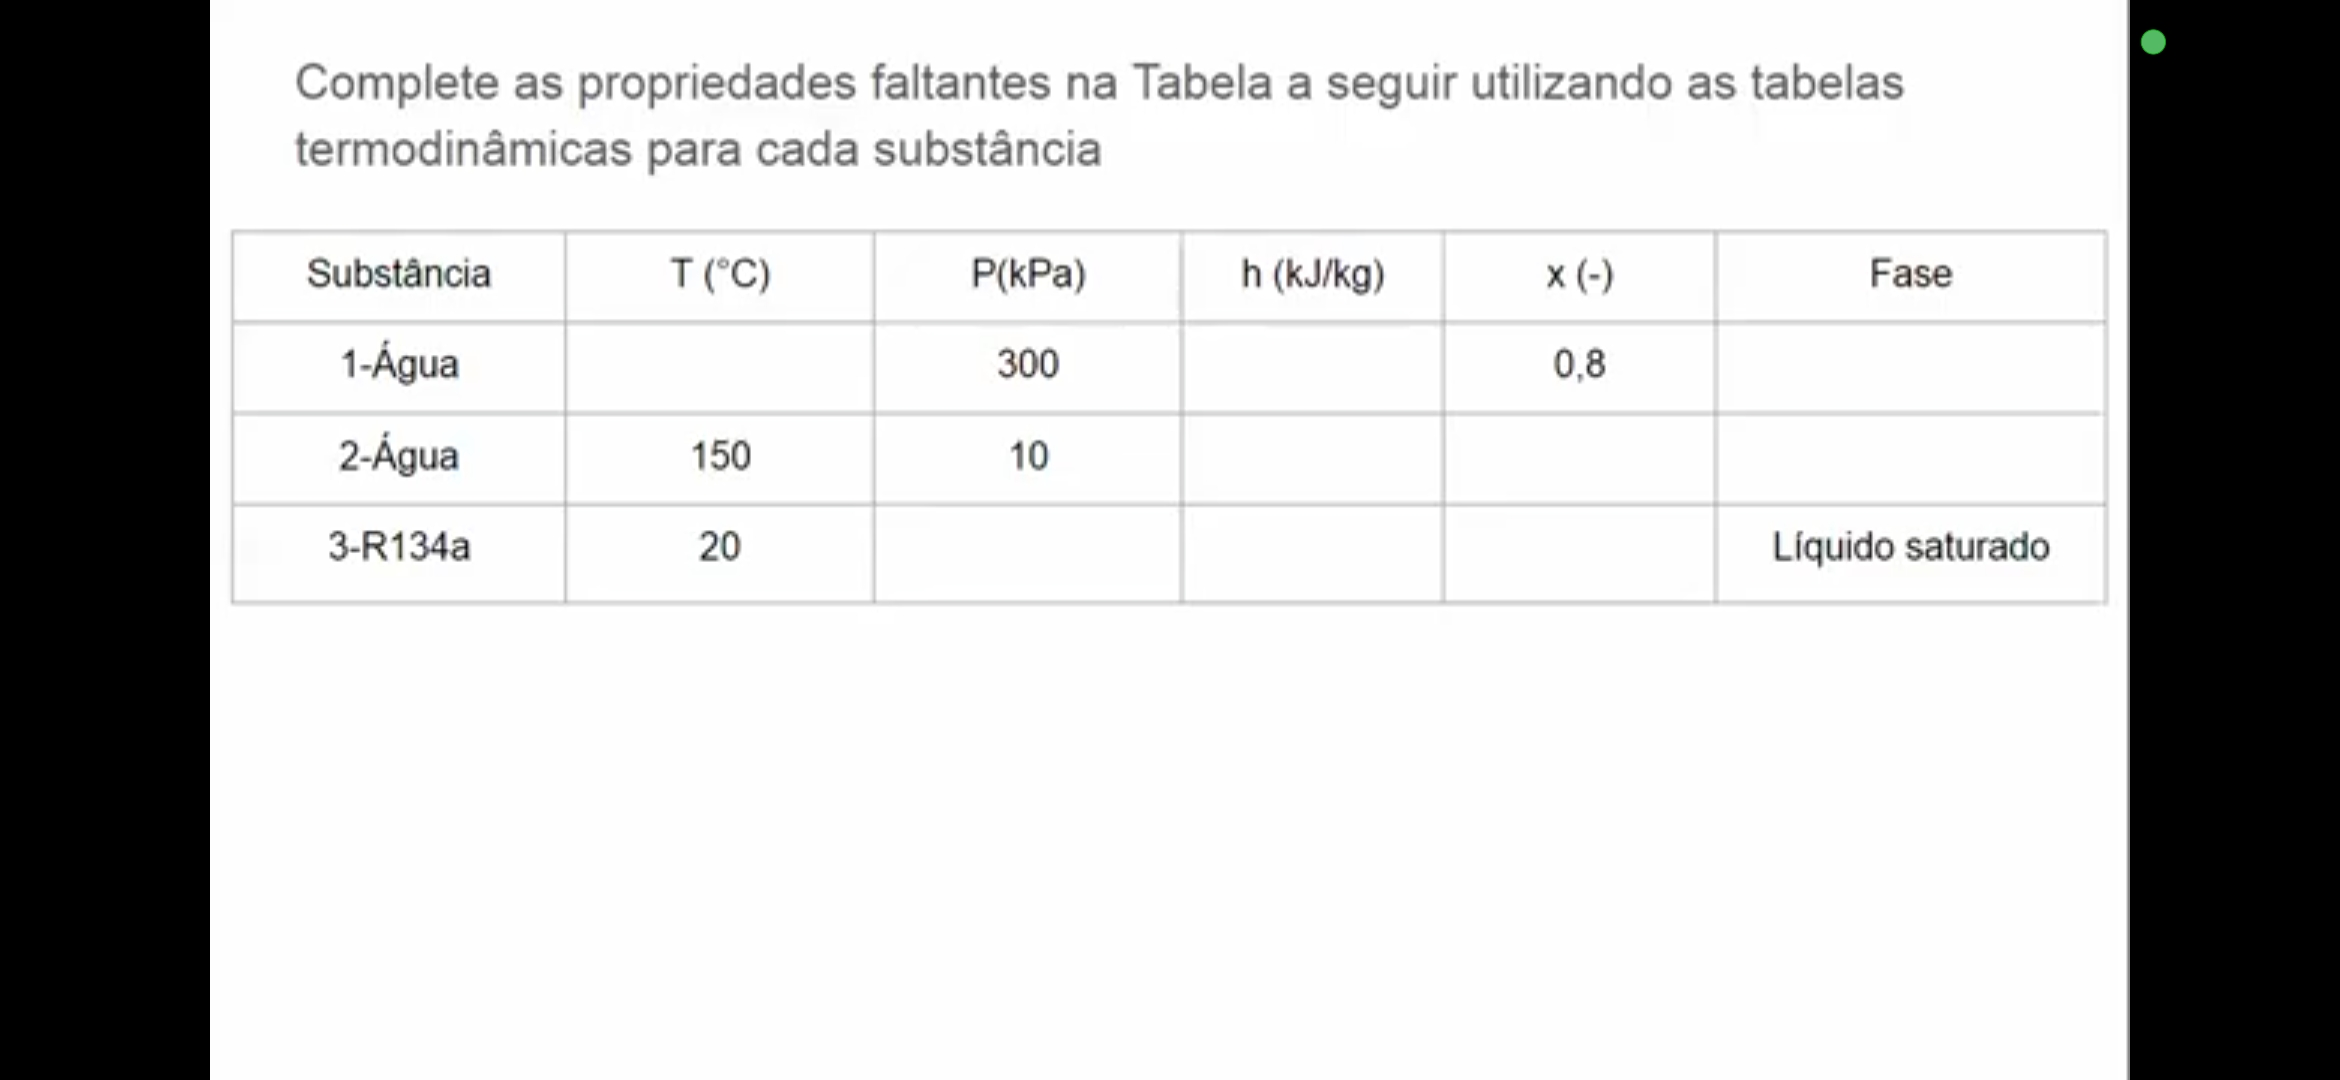
\includegraphics[width=1\linewidth]{table.jpg}
    \caption{tabela da questão}
    \label{fig:tabela da questão}
  \end{figure}
\subsection{library coolprop}
\begin{lstlisting}
P1 = 300E3 #Pa
x1 = 0.8
T1 =  PropsSI("T","P",P1, "Q", x1, "water") - 273.15 # A primeira letra  e dimensao 
#que eu quero , as duas proximas, sao as dimensoes que eu vou informar, e o 
#nome da substancia
Tcrit = PropsSI("Tcrit", "water") 
print (f"A temperatura da agua nessas condicoes e {T1:.2f} celsius")
print(f"A temperatura critica da agua  e {Tcrit:.2f} celsius")
\end{lstlisting}

\subsection{definições}{Fração de vapor}\\
Quando a qualidade (ou fração de vapor) é negativa, isso geralmente indica que a substância está em um estado de mistura de líquido-vapor, ou seja, está em um estado bifásico, com uma parte líquida e outra de vapor.

A qualidade (x) é definida como a fração de massa que está na fase de vapor em relação à massa total. Quando x é negativo, significa que a quantidade de líquido presente é maior do que a quantidade de vapor esperada para a condição de pressão e temperatura especificada.

Existem algumas situações em que isso pode ocorrer, como:
\begin{itemize}
    \item Sobreaquecimento: A temperatura está acima da temperatura de saturação correspondente à pressão especificada, mas a pressão ainda está abaixo da pressão de saturação. Nesse caso, parte da substância pode estar no estado de vapor, enquanto o restante está superaquecido.

    \item Sub-resfriamento: A temperatura está abaixo da temperatura de saturação correspondente à pressão especificada, mas a pressão está acima da pressão de saturação. Isso pode ocorrer quando a substância está sendo comprimida ou resfriada rapidamente.

\end{itemize}


Seria útil verificar os valores de pressão e temperatura fornecidos e garantir que estão dentro dos limites adequados para a substância e para o modelo termodinâmico utilizado. Além disso, verificar se há outros fatores que possam influenciar a qualidade da substância nas condições específicas em questão.

\end{document}

\item \textcolor{green}{}
\item \textcolor{red}{}
\item \textcolor{blue}{}
\noindent\rule{\textwidth}{0.4pt}
\subsection*{}
